\documentclass{llncs}
\usepackage{makeidx}
\usepackage{amsmath}
\usepackage{amsfonts}
\usepackage{amssymb}
\usepackage[spanish]{babel}
\usepackage{graphicx}

%opening
\title{\large\huge Super Proyecto\\de \\ IA + Compilación + Simulación}
\author{Integrantes: \\ Julio José Horta C312 \\Javier Villar Alonso C311 \\ Dayron Fernández C311}

\begin{document}
	
\maketitle

\newpage

\section{General}
En este trabajo nuestro objetivo es simular el desarrollo de la vida en cualquier planeta y acercarnos lo más posible a la forma adaptativa de las especies ante los cambios naturales, la evolución de la misma y la competencia entre estas tal cual como ocurren en nuestro mundo natural.
\newline
\newline
Esto tiene como objetivo reunir datos estadísticos del comportamiento natural de las especies para asi asimilar mejor su expansión natural y la adaptabilidad en el mundo, asi como que tan dañino pueda ser un fenómeno en específico. 


\section{Aplicación}

\begin{figure}
	\centering
	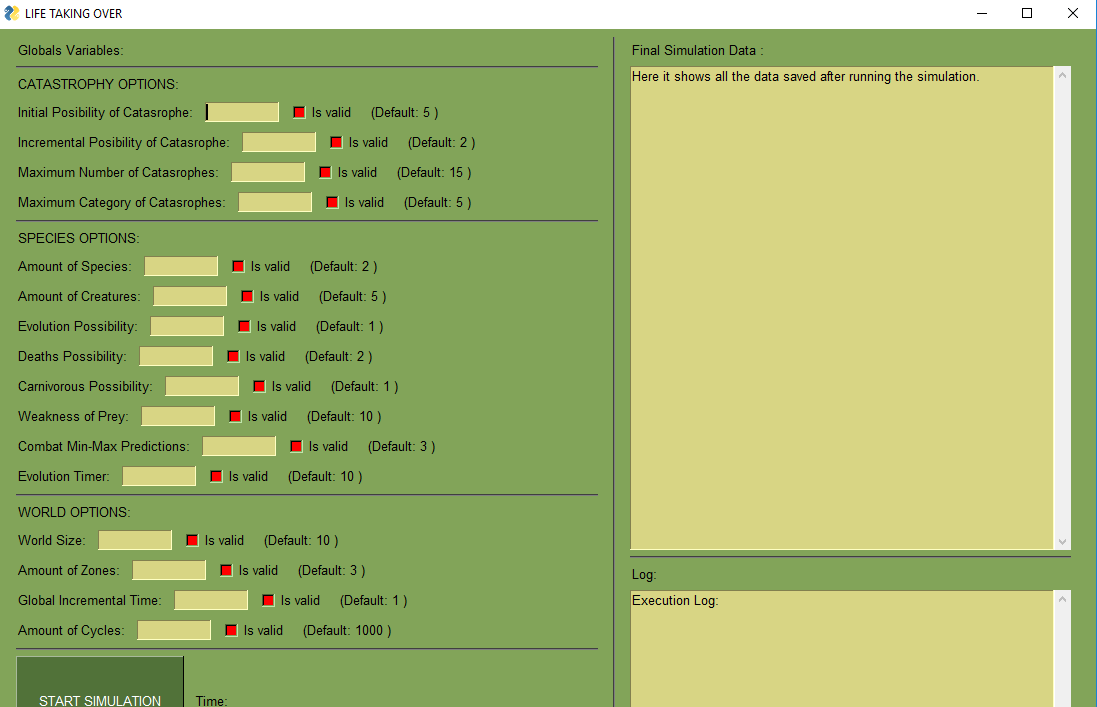
\includegraphics[width=0.7\linewidth]{imagenesapk/HomeForm}
	\caption{}
	\label{fig:homeform}
\end{figure}

Creamos un pequeño form para poder modificar parametros de la aplicación. Este aplicación permite cambiar parámetros a la simulación para poder interactuar con ellas y ver resultados atendiendo al número de ocurrencia de acciones, cantidad de individuos nacidos, cantidad de muertes, entre otras.

\begin{figure}
	\centering
	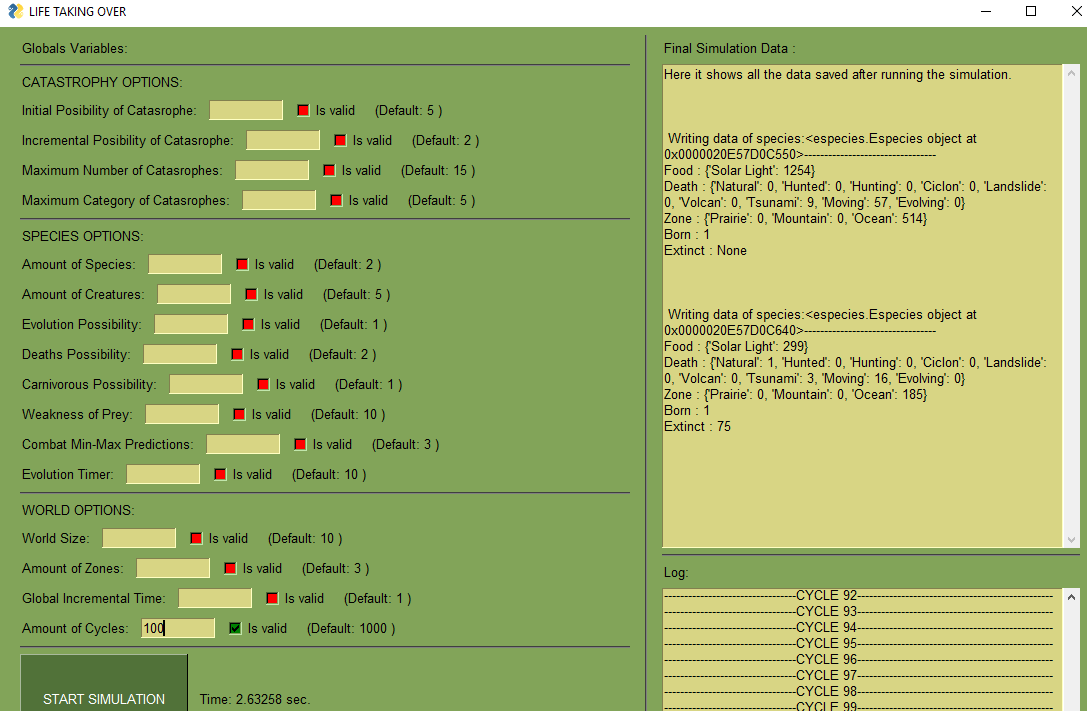
\includegraphics[width=0.7\linewidth]{imagenesapk/ResultForm}
	\caption{}
	\label{fig:resultform}
\end{figure}

\section{Código}

\subsection{Mapa}
\begin{figure}[]
	\centering
	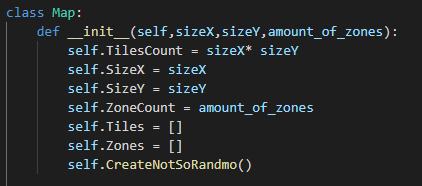
\includegraphics[width=0.7\linewidth]{imagenes/mapa}
	\label{fig:mapa}
\end{figure}

El mapa es el mundo en el que vamos a llevar a cabo la simulación. Este mundo consta de una matriz donde establecemos el tamaño de nuestro mapa de acuerdo al largo y ancho, a lo cual nombramos tamaño del eje X y tamaño del Eje Y respectivamente, además de mandar la cantidad de zonas que crearemos genéricamente para nuestro mundo
\newline
\newline
Para recorrer nuestro mapa usaremos una matriz adecuada a los tamaños mandados, en el que cada una de las coordenadas es un Tile (la cual estaremos explicando posteriormente). También llevaremos como variable cada una de las zonas existentes en el mundo de forma independientes aunque sean del mismo tipo
\newline
\newline
Este mapa está diseñado para que no existan límites ya que tiene más sentido para nuestra simulación que sea un entorno circular antes que cuadrático

\subsection{Zones}
\begin{figure}
	\centering
	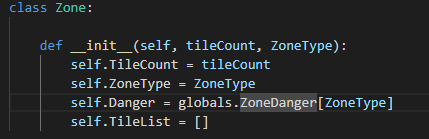
\includegraphics[width=0.7\linewidth]{imagenes/Zona}
	\label{fig:zona}
\end{figure}


Una zona es un ambiente natural que consta de un conjunto de tiles que expresan la expansión en la que vivirán nuestras especies.
\newline
\newline
Estas constan de una variable Tiles que agrupará en un array todos los tiles que corresponden a la zona, un string que nos diga el tipo de zona, una variable danger que nos expresará cuan peligroso es la zona, y por último un contador de cuantos tiles hay en la zona


\subsection{Tiles}
\begin{figure}
	\centering
	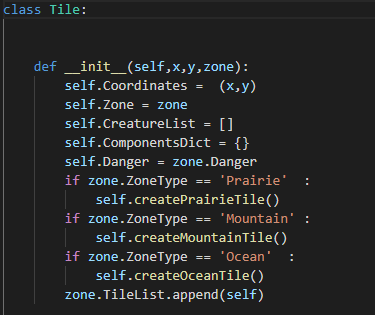
\includegraphics[width=0.7\linewidth]{imagenes/Tile}
	\label{fig:tile}
\end{figure}

Un tile es una ubicación de una zona natural del mapa en el que los individuos de las diferentes especies interactúan en ella, ya sea en busca de alimentos, de compañeros de una especie o la caza de estos para alimentarse.
\newline
\newline
Estos tiles constan de las coordenadas de ubicación de la zona, las cantidad de criaturas que se encuentran en ella, los recursos disponibles en ella guardados en una variable llamada ComponentsDict

\subsection{Especies}
\begin{figure}
	\centering
	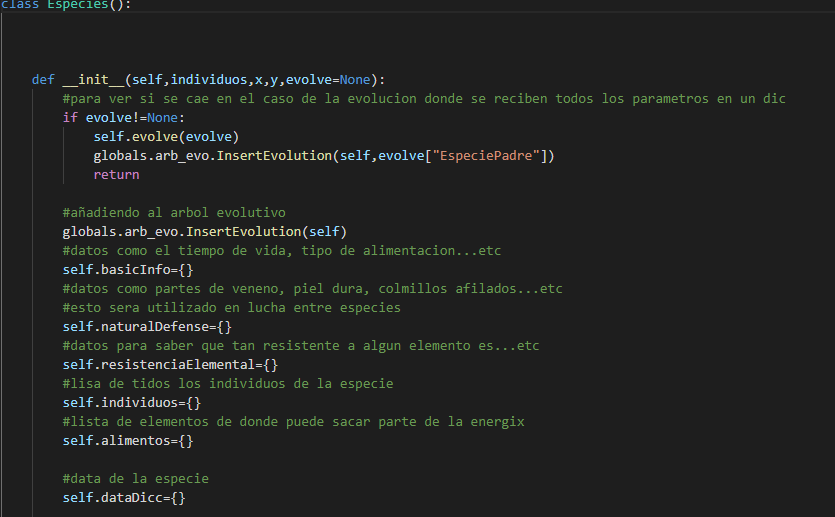
\includegraphics[width=0.7\linewidth]{imagenes/Especie}
	\label{fig:especie}
\end{figure}

Para poder crear una interacción en el mundo creado decidimos añadir especies para que formen parte de este mundo, estos se caracterizarán por individuos que realizarán funciones básicas para vivir en ese mundo.
\newline
\newline
Este recibe un número que especifica la cantidad de individuos que se quiere para añadirlos en una posición determinada en el mapa, para ello les mandaremos también las coordenadas en donde se quiere ubicar. Luego también mandaremos una variable evolve que en caso de no mandarlo se interpretará como que no es posible que evolucione
\newline
\newline
Estas especies serán insertadas en un árbol de evolución para crear un árbol geneológico para tener una relación evolutiva de cada uno se registrarán
\newline
\newline
Luego tenemos unos diccionarios que se encargan de guardar información de una especie. Entre ellas tenemos el ´basicinfo´ que se encargará de guardar informaciones básicas de una especie, como lo es el nombre, tipo de células, entre otros.
\newline
\newline
Otro de los diccionarios es el naturaldefence, en el cual guardaremos las características numéricas de la especie, como lo es la vida, la percepción para saber cuantas casillas puede ver a su alrededor, inteligencia, tiempo de reproducción, cualquier estadística que tenga que ver con la forma de comportarse en el mundo
\newline
\newline
También tenemos un diccionario de alimentos que nos permite guardar que acostumbra a comer cada animal y cuanta energía recibe al comer dicho alimento
\newline
\newline
Por último tenemos un diccionario de data que es para guardar información de interés de la especie, como por ejemplo la forma que murió cierto individuo, que han comido los individuos, cuales fue los que más comió, y otras informaciones de interés que queramos consultar en la simulación
\newline
\newline
Como antes informamos las especies son un grupo de individuos, por lo que miremos como creamos esta clase

\subsection{Individuos}
\begin{figure}
	\centering
	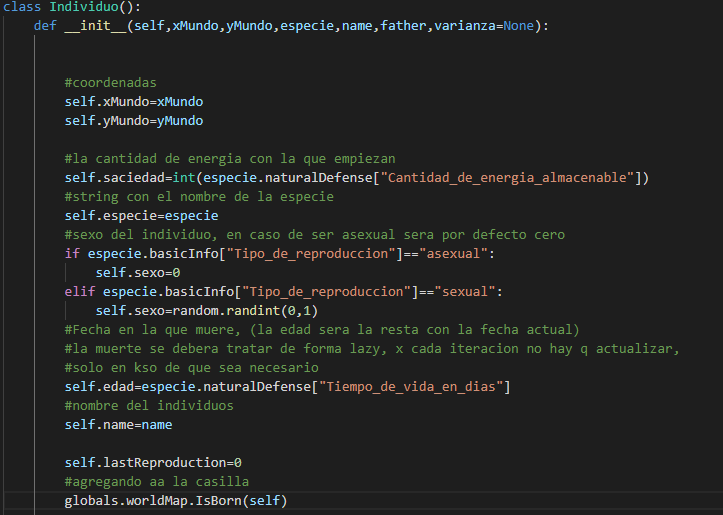
\includegraphics[width=0.7\linewidth]{imagenes/Individuo}
	\label{fig:individuo}
\end{figure}

Los individuos son entidades particulares de una especie que tienen los valores cercanamente iguales a los establecidos en la especie, así podemos establecer una diversidad entre varios individuos.
\newline
\newline
Estos individuos serán creados mediante las coordenadas XY de mundo, su especie padre, nombre de individuo y una varianza que servirán para la evolución
\newline
\newline
También se inicializará en el constructor variables como la saciedad para saber la cantidad de energía que presenta este individuo, la edad, además de las naturaldefence del propio individuo que son parecidas a las del padre pero con una probabilidad de ser diferente.
\newline
\newline
Entre las funciones añadimos un método \textbf{breed} para simular la simulación, en el cual si un individuo tiene reproducción asexual se realiza una clonación, mientras que si tiene reproducción sexual entonces verificamos si la especie femenina es fertil.
\newline
\newline
Cada individuo puede moverse de acuerdo a una velocidad traducida en la cantidad de casillas a poder moverse, este se moverá de acuerdo a la inteligencia del individuo
\newline
\newline
Cuando tiene inteligencia menor que 2 solo podrá moverse para un lado (permitiendo diagonal).
\newline
\newline
Tenemos también un movimiento random y un movimiento inteligente.
\newline
\newline
El move recibe un variable mapa que se destaca en un diccionario que tiene varios mapas adentro donde nos podemos mover.
\newline
\newline
Cada vez que el individuo se mueva comprobará si el individuo se muere al moverse o incluso si se muere en la posición en donde estaba por el nivel de peligrosidad de la zona a la que se movió
\newline
\newline
Otra función que pueden hacer los individuos es \textbf{eat}, la cual radica registrar una lista de alimentos que se encuentran en la lista del tile y revisa si se encuentran los alimentos que puede comer en esa zona para luego saciar su energía en caso de encontrar alguno. Es importante destacar que cada alimento consumido será eliminado de la zona
\newline
Adicionalmente añadimos el string cazador que permite a los individuos cazar a otras especies, por lo que tratará de buscar un individuo que esté por su zona que se pueda comer de forma inteligente, es decir, que el enemigo sea factible como objetivo a comer en cuanto a sus características de especie comparados a la de este cazador.
\newline
Una vez identificado y encontrada una presa se efectuará un combate, en el cual si el individuo muere se manda a matar al cazador, si la presa muere entonces se manda a morir a la presa y el cazador recupera energía. También las presas pueden huir, por lo que no necesariamente habrán ganadores.
\newline
\newline
También tenemos la función \textbf{die} que es la que se encarga de mandar a morir al individio y a realizar todas las modificaciones que implican eliminarlo, como es modificar los individuos en el mapa, modificar los individuos de nuestro diccionario de especies, entre otros.
\newline
\newline
Por ultimo tenemos la función resolveIteration que es la función que se encarga de ejecutar las acciones de mover y comer por parte del individuo
 

\subsection{Fenómenos}
\begin{figure}
	\centering
	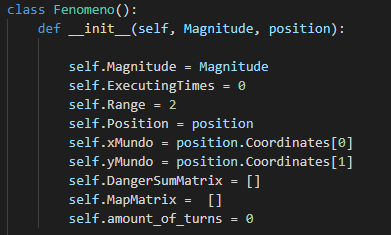
\includegraphics[width=0.7\linewidth]{imagenes/fenomeno}
	\label{fig:fenomeno}
\end{figure}

Los fenómenos los incorporamos como los accidentes meteorológicos que ocurrirán en nuestro mundo para afectar el número de las especies y los recursos que existen en la zonas, además de la peligrosidad en cada zona que afectará al movimiento de cada criatura de acuerdo a la percepción
\newline
\newline
Estos tienen como parámetros la magnitud de escala del fenómeno que establece el nivel de propagación y peligrosidad de este, las coordenadas de ubicación donde se generará dicho fenómeno, las matrices de percepción y daño que alcanza el fenómeno, la posición, el rango, la cantidad de turnos y el tiempo de duración
\newline
\newline
Estos fenómenos tienen una probabilidad de ocurrir de acuerdo a la zona en la que esté de acuerdo a una curva de probabilidad, la cual va cambiando de acuerdo al tiempo de ocurrencia de los fenómenos de forma incremental, es decir, mientras más tiempo demore en ocurrir un fenómeno va incrementando su probabilidad. Esta probabilidad de aparición se encargaría nuestra heurística, la cual calculará un random para saber si ocurrirá una catástrofe para luego calcular bajo unas coordenadas randoms el valor de una distribución normal para poder saber que fenómeno se generará en ese momento.

\subsection{Misc}
El misc incorpora todos los métodos útiles que necesitemos para nuestro trabajo, esto incluye las operaciones de matrices y las inteligencias artificiales implementadas en nuestro trabajo, la cual estaremos hablando un poco en estos momentos.

\begin{figure}
	\centering
	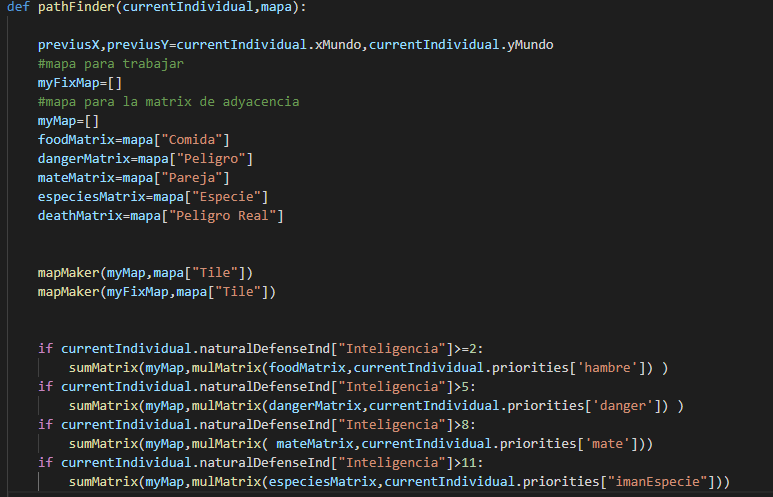
\includegraphics[width=0.7\linewidth]{imagenesMisc/pathfinder1}
	\label{fig:pathfinder1}
\end{figure}
\begin{figure}
	\centering
	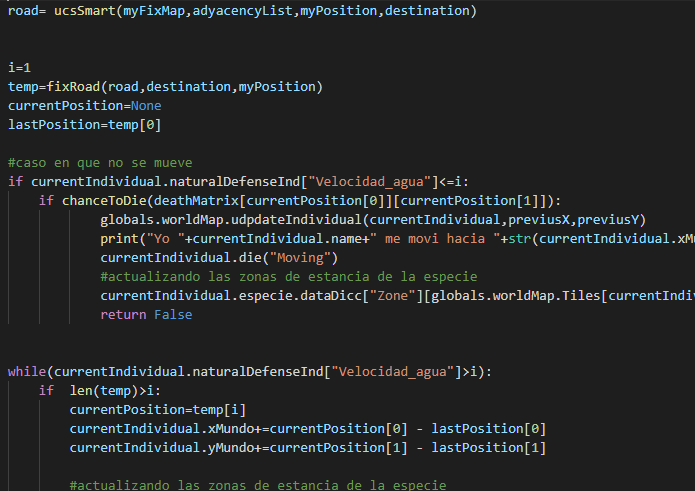
\includegraphics[width=0.7\linewidth]{imagenesMisc/pathfinder2}
	\label{fig:pathfinder2}
\end{figure}

Al partir del método pathfinder empezaremos a trabajar el movimiento inteligente. Este recibe una instancia de individuos y un mapa que es un diccionario que contiene vario mapas de acuerdo a la percepción del individuo, es decir, si tienes percepción 1 entonces tomaremos el mapa que resulta de moverse en 1 a todas las casillas que impliquen solo dar un paso, incluyendo el movimiento adicional.
\newline
\newline
Luego de definir el rango de percepción del mapa evaluamos en cada matriz los diferentes mapas mandados en el diccionario bajo esa percepción sobre donde hay comida, donde hay peligro, parejas y especies, la cual identificaremos como 1 a los que más le interese al individuo, excepto peligro real que nos dará el valor real. Estos mapas serán los criterios de nuestro movimiento inteligente, la cual dependiendo de la inteligencia del individuo tomará cada criterio, de las cuales lo más complicado que puede prever es el moverse a donde está más concentrada su especie.
\newline
\newline
Luego sumamos los pesos de la matriz para luego tener un matriz pesada para hacer el A* para buscar la casilla que tenga con el mejor valor para tratar de llegar allí

\begin{figure}
	\centering
	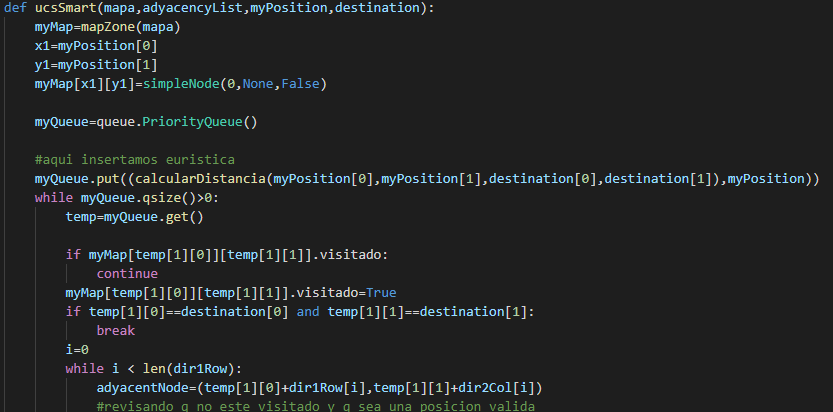
\includegraphics[width=0.7\linewidth]{imagenesMisc/UcsSmart}
	\caption{}
	\label{fig:ucssmart}
\end{figure}

El método A*, la cuál en nuestro trabajo lo nombramos como UcsSmarth. Este método toma un mapa y unos pesos para la arista del grafo que empieza a revisar la aristas por el orden de prioridad con una heurística de distancia Euclediana. Todas nuestras casillas están pesadas entre 1 y 5, el camino más cercano de una casilla a otra solo puede ser 1 por lo que nuestra heurística Euclediana es optimista ya que no habrá camino más corto que la línea recta.
\newline
\newline
Se van llenando los nodos hasta llegar a la casilla destino, por lo que devolveríamos el grafo resultante y el padre, con el que podremos ir construyendo el camino.
\newline
\newline
Este ucsSmart funciona con un drijktra, un método estudiado en estructura de datos para determinar la longitud del camino más corto entre dos vértices de un grafo ponderado simple, conexo y no dirigido con n vértices.

\begin{figure}
	\centering
	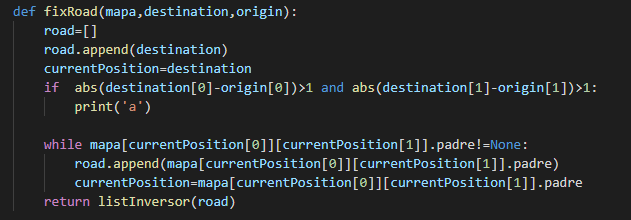
\includegraphics[width=0.7\linewidth]{imagenesMisc/FixRoad}
	\label{fig:fixroad}
\end{figure}

Luego de tener el camino correcto llamamos al método fixroad que se encarga de ir regresando desde el nodo final hasta el inicial por los padres para saber el camino a tomar.
\newline
\newline
Luego por cada paso que se da comprobaremos si por moverte llega a morirse nuestro individuo, ya que existe una probabilidad de llegar a morirse al moverse y al quedarse en una casilla dependiendo del peligro real de cada casilla, dando respuesta a la razón del por qué llevamos la matriz de peligro. 
\newline
\newline
Ahora hablaremos de la inteligencia artificial de combate:

\begin{figure}
	\centering
	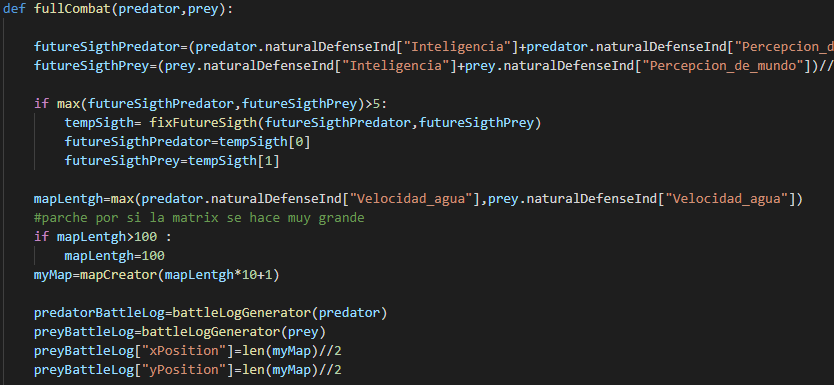
\includegraphics[width=0.7\linewidth]{imagenesMisc/fullCombat}
	\label{fig:fullcombat}
\end{figure}

Esta caso nosotros lo iniciamos con el método llamado fullcombat, el cual da inicio a la situación de combate que se efectuarán entre dos individuos, depredador y presa. Tendrán una ubicación en el mapa donde el depredador andará en el medio del mapa y la presa en una esquina. El mapa tendrá un tamaño de acuerdo al tamaño entre las dos velocidades entre los dos individuos x 10, para que al menos haya 10 turnos.
\newline
\newline
Para llevar a cabo el combate haremos un Min-max donde llevaremos unos diccionarios de registros llamados battlelog para cada individuos donde registraremos la vida, lenteos, daños y otros elementos.

\begin{figure}
	\centering
	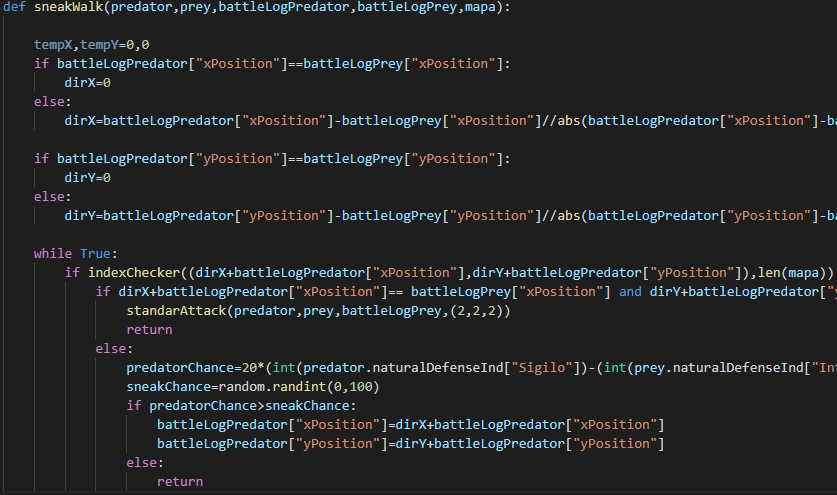
\includegraphics[width=0.7\linewidth]{imagenesMisc/sneakwalk}
	\label{fig:sneakwalk}
\end{figure}

Una vez seteados los elementos empieza el combate, donde lo primero que haremos es acercar a la presa en el combate con un método llamado sneakwalk, en el que se recibe el sigilo del cazador y se lleva contra la inteligencia y percepción de la presa promediada, mientras mayor sea el sigilo comparado con las estadísticas antes dicha del cazador, mayor ventaja tendrá el cazador, de lo contrario la tendrá la presa.
\newline
\newline
El cazador empezará a moverse una casilla a la vez, y se hará una distribución normal donde si se cae dentro de la zona segura para el cazador, entonces la presa no lo descubrirá y podrá moverse de nuevo. Si en algún momento es descubierto, detenemos el método y retornamos, obteniendo así las nuevas posiciones en el registro. En caso de que el cazador llegue al objetivo entonces la presa recibirá un golpe de mucho daño por parte del cazador.
\newline
\newline
Una vez que llegue a ser descubierto el cazador y aun le quede vida a la presa realizaremos el Min-Max, llamando a los método CombatTurnPredetor y CombatTurnPray en dependencia si eres depredador o presa.

\begin{figure}
	\centering
	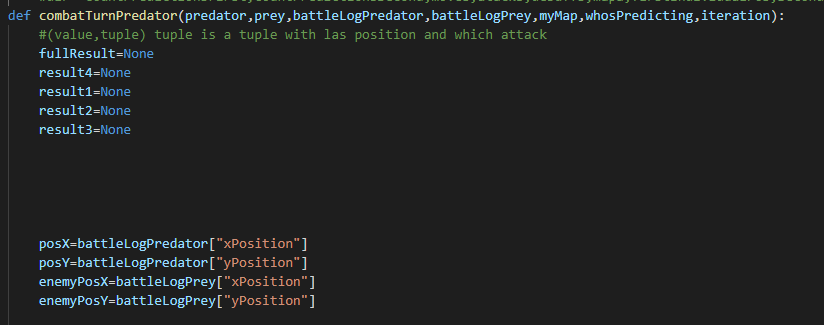
\includegraphics[width=0.5\linewidth]{imagenesMisc/CombatTurnPredator}
	\label{fig:combatturnpredator}
\end{figure}
\begin{figure}
	\centering
	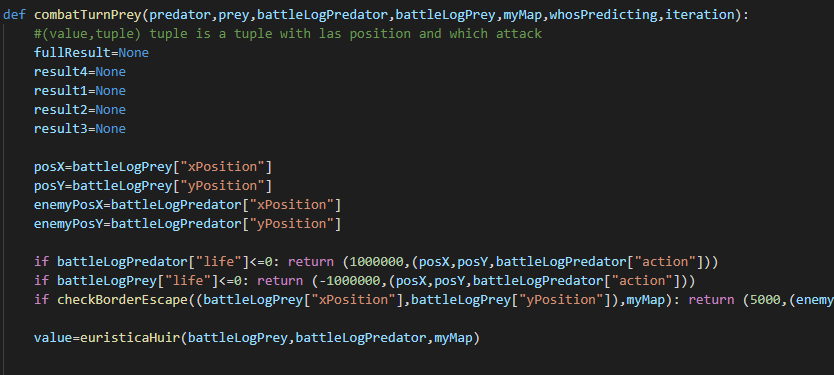
\includegraphics[width=0.5\linewidth]{imagenesMisc/CombatTurnPray}
	\label{fig:combatturnpray}
\end{figure}


El cazador va a tener varias casillas a moverse y tendrá tres posibles ataques a realizar: ¨ataque normal¨, ¨ataque crítico¨ y ¨ataque de lenteo¨, atendiendo a esto el CombatTurnPredetor buscar todas las casillas a las que se puede mover y si tiene posibilidad de dar uno de los 3 golpes antes dicho. En caso de moverse, para evitar análisis de casos exponenciales usamos una variable global llamada tempPredictions y utilizamos una poda por debajo para evitar esto mediante el uso de la heuristicahunt para buscar un acercamiento del depredador hacia la presa.
\newline
\newline
En caso de CombatTurnPray se basa parecido al CombatTurnPray, donde nos interesa más buscar rutas de escape mediante nuestra heuristica de huir si es que la presa sigue viva después de la acción del depredador.

\begin{figure}
	\centering
	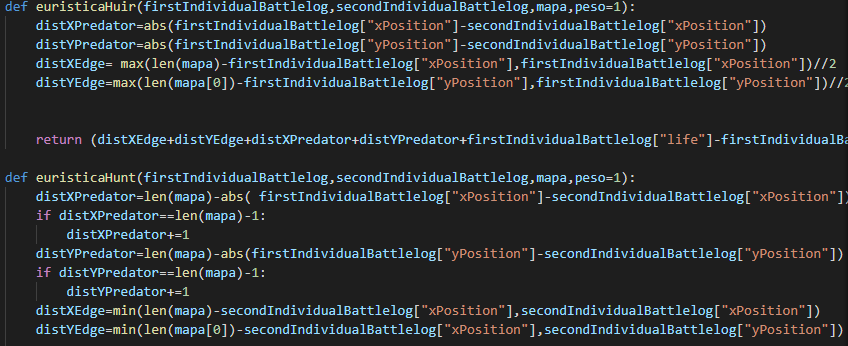
\includegraphics[width=0.7\linewidth]{imagenesMisc/HeuristicHH}
	\label{fig:heuristichh}
\end{figure}

Una vez mandadas las opciones, tomamos el valor que nos otorga el min-max por tomar cierta opción o cierta acción y nos quedamos con el mayor. Para ello tenemos una heurística para saber que tan favorable es para el cazador y que tan favorable es la heurística y nos quedamos con el mejor de los resultados.
\newline
\newline
Como controlamos la duración del combate?
\newline
\newline
Cuando llamamos la primera vez a CombatTurnPredetor o a CombatTurnPray, en dependencia de quien predijo el combate, y mandamos una cantidad de turnos a revisar re escalando mediante la comparación de las inteligencia de los dos individuos.
\newline
\newline
El método findPray se encarga de buscar una presa que no sea difícil de matar, no lo mate y que le permita llenarse. Esto se logra buscando el de menor características que le de mayor cantidad de vida, dependiendo del hambre que tenga el individuo

\end{document}
